
\documentclass[conference]{IEEEtran}
\usepackage{amsmath} 
\usepackage{tikz}
\usepackage{graphicx}  
\usepackage{textcomp}
\usepackage{amssymb}
\usepackage{enumitem}
\usepackage{pgf}
\usepackage{url}
\usepackage{csvsimple}
\usepackage{booktabs}


\begin{filecontents*}{timespent.csv}
number,time(m),time (m),time (m),time (m),time (m),time (m),time (m),
0,0,0,1,4,7,8,8
1,5,5,3,0,6,6,7
2,3,3,5,6,5,10,10
3,7,7,2,9,9,9,10
4,3,3,3,6,7,8,8
5,4,4,3,5,5,7,7
6,1,1,8,7,6,8,7
7,1,1,0,9,6,8,8
8,3,3,6,8,5,5,7
9,1,1,10,6,8,6,8
10,6,6,1,6,5,5,8
11,2,2,1,2,6,10,10
12,2,2,7,6,9,5,9
13,2,2,2,9,8,5,10
14,6,6,4,4,9,7,10
15,7,7,6,4,10,8,7
16,4,4,6,1,8,7,9
17,2,2,6,8,9,5,9
18,0,0,0,3,5,6,7
19,1,1,1,1,6,9,7
20,0,0,9,3,6,9,9
21,0,0,0,4,5,10,8
22,9,9,8,2,10,7,10
23,4,4,0,3,10,5,10
24,2,2,5,0,10,9,7
25,5,5,1,0,8,5,7
26,10,10,6,7,6,8,10
27,5,5,0,7,6,6,10
28,4,4,4,8,5,6,7

\end{filecontents*}




\setlist{  
  listparindent=\parindent,
  parsep=0pt,
}

\newlength{\bibitemsep}\setlength{\bibitemsep}{.2\baselineskip plus .05\baselineskip minus .05\baselineskip}
\newlength{\bibparskip}\setlength{\bibparskip}{0pt}
\let\oldthebibliography\thebibliography
\renewcommand\thebibliography[1]{%
  \oldthebibliography{#1}%
  \setlength{\parskip}{\bibitemsep}%
  \setlength{\itemsep}{\bibparskip}%
}

\usepackage{xspace}

\newcommand\nd{\textsuperscript{nd}\xspace}
\newcommand\rd{\textsuperscript{st}\xspace}
\newcommand\nth{\textsuperscript{th}\xspace}
\usetikzlibrary{shapes.geometric, arrows}

\ifCLASSINFOpdf
 
\else

\fi

%\hyphenation{}

\begin{document}
\title{ALFRED - A Conversational Shopping Assistant }


\author{
\IEEEauthorblockN{Pushkaraj Joshi}
\IEEEauthorblockA{Department of Computer Engineering\\
Ramrao Adik Institute of Technology\\
Navi Mumbai, India}\\   
%<------ Line breaks in the current column
\IEEEauthorblockN{Saurabh Jain}
\IEEEauthorblockA{Department of Computer Engineering\\
Ramrao Adik Institute of Technology\\
Navi Mumbai, India}
\and

\IEEEauthorblockN{Arvind Mishra}
\IEEEauthorblockA{Department of Computer Engineering\\
Ramrao Adik Institute of Technology\\
Navi Mumbai, India} \\[0cm]  
%<------- Extra vertical space
\IEEEauthorblockN{Prathmesh Gunjgur}
\IEEEauthorblockA{Department of Computer Engineering\\
Ramrao Adik Institute of Technology\\
Navi Mumbai, India}
\and

\IEEEauthorblockN{Siddhant Mohapatra}
\IEEEauthorblockA{Department of Computer Engineering\\
Ramrao Adik Institute of Technology\\
Navi Mumbai, India}\\        
         %<-----------
\IEEEauthorblockN{Puja Padiya}
\IEEEauthorblockA{Department of Computer Engineering\\
Ramrao Adik Institute of Technology\\
Navi Mumbai, India}
}

% make the title area
\maketitle


% As a general rule, do not put math, special symbols or citations
% in the abstract
\begin{abstract}
Online shopping is an enormous domain, gaining wide popularity about 20 years ago. Industry leaders like Amazon and Flipkart have millions of daily active users. The ease of payments and on demand logistics means online shopping is here to stay, and may get even more dominant with time. The proposed system intends to tap into this growing market, using advances in the field of Machine Learning, Expert Systems and Natural Language Processing. The proposal aims to enhance the user\textquotesingle s online shopping experience and deliver a mobile first system towards a fully automated, intelligent shopping assistant that uses personalized recommendations and a natural interface to make online shopping convenient.
\end{abstract}

% no keywords

% creates the second title. It will be ignored for other modes.
\IEEEpeerreviewmaketitle



\section{Introduction}
% no \IEEEPARstart
Computer systems can now understand natural language, inching close to mimicking actual conversational human interaction. Modern smartphones are suited for conversational interfaces and online shopping can take advantage of this feature set, thus creating a rich experience for the users.

Conversation based agents pose several challenges, chief of which is the understanding and manipulation of natural language. An idea can be conveyed in many ways; its proper interpretation requires a robust and fault tolerant framework. 

To accurately understand a user\textquotesingle s text or voice input, the system makes use of Natural Language Processing. NLP is a sub-field of computer science and it enables natural interactions with machines. Conversational Interfaces make use of NLP and bi-variate attention models to construct natural responses to user input to mimic a real world conversation flow. Conversational UIs have ushered computer systems away from cryptic interfaces\cite{be1}. 

Once the user has given the input, the system needs to deliver a personalized result. It achieves the same using an optimization technique called query personalization. It lowers the computational cost of performing search and dynamically reduces the scope of open ended queries with the help of available profile data, cutting a large portion of the search space. Query personalization is often used hand in hand with recommendation systems because when dealing with large number of items, it makes sense to remove irrelevant data to arrive at suitable recommendations for the user. 

Recommendation systems are information filtering systems that seek to remove irrelevant data with the aim of arriving at suitable recommendations for a user. Recommendation systems allow for filtering and ranking of data that is relevant to the given user, on the basis of their profile. They are particularly useful when there are a large number of alternatives which can be difficult to search efficiently and can help reduce transaction costs for online shopping.

A personal assistant that combines language understanding, smart searching and recommendations via a natural interaction model will be a big step up from the existing approach to online shopping. Such an assistant will deliver on the promise of intelligent systems and present a compelling example of how such advancements can be utilized to deliver solutions that upgrade everyday experiences. 

The rest of the paper is structured as follows:
Section ``Related Work''   presents the relevant literature related to the problem domain. We take a deep dive and analyse the research carried out before us, arriving at a problem statement that allows us to proceed with the development of the system. Section ``Proposed System" introduces the architecture and flow of the proposed system for the defined problem statement. Section ``Proposed Methodology" presents low level implementation details and deals with the proper working of the proposed system. Section ``Results and Discussion" presents a commentary on the results obtained and the comparison with existing approaches. Finishing remarks and possible future work is presented in the Section ``Conclusion".
\section{Related Work}
\label{sec:2}

Researchers have come up with different methods that deal with different aspects of conversation based agents. V. Zue, Stephanie S. \textit{et al.} in \cite{be2} have taken a domain specific approach, drawing responses from a vocabulary corpus, with the system open only to inputs that are within the domain of the problem statement. For inputs not within the domain, the system incorporates error handling to maintain conversation flow. The response from the system, however, is very structured and decreases qualitatively over time, with increasingly verbose and out of context responses on repeated non-domain queries. This can be tackled by incorporating attention models such as seq2seq \cite{be3} which generate responses character by character using probability distributions on input data.

In order to make conversational interfaces feasible for online shopping, they need to have domain specific functional knowledge so they are able to understand and respond to queries, as put forward by J. Chai \textit{et al.} in \cite{be4}. This allows the system to ensure that the flow of the conversation is maintained in the right direction.
 
Quarteroni and Manandhar in \cite{be5} have put forward an approach to an open domain question answering(QA) system that can identify whether the input question has a factoid answer or not and can then proceed to process it differently. Higashinaka \textit{et al.} in \cite{be6} have devised a system that is an open domain, non-task oriented conversational system. The core emphasis of their approach has been on generating and understanding utterances. Following discourse theory (Grosz and Sidner, 1986), the authors devised an architecture that uses intention (intentional structure), topic (state) and content (linguistic structure) to understand input and generate appropriate utterances. This, in turn, allows them to build a general conversational agent that is capable of carrying out conversations similar to a human.

Bonnie Chantarotwong in \cite{be8} has demonstrated an approach where the chatbot is trained on a corpus of real world conversation data using Conditional Frequency Distributions (CNFs). This was done to allow the chatbot to come up with realistic sounding responses rather than stitching together the most important words in a sentence. This approach, called Case Based Reasoning, means that the responses from the chatbot are restricted only to the training corpus.  An approach to overcome this has been described by A. Sriram \textit{et al.} in Cold Fusion \cite{be9} which utilizes a language model during training, learning to understand its specific information and capturing only the information that is relevant to the generation of the target sequence.

Koutrika in \cite{be10} puts forward an architecture that allows queries to be modified dynamically allowing for personalized recommendations that are needed to fulfilling the promise of a truly intelligent assistant. By using a locally stored user profile to augment the incoming query, the proposed architecture is able to ensure that minimum criteria of a user s top preferences are met, paving the way for truly personalized recommendations. The recommendation system adopts two approaches to generate personalized results: collaborative filtering and modelling past customer behaviour. Prassas and Pramataris in \cite{be11} have put forward an architecture which takes into account a user's past history to determine the kind of products that they might like. 

This approach is also complimentary to the emphasis on collaborative filtering in \cite{be12} which uses a similarity function to determine similar users within its user neighbourhood. This in turn is useful as a neighbour�'s graph of purchased items can be used to generate recommendations for the user. 

The literature studied above is essential towards understanding how existing systems work. To truly deliver on the promise of the assistant, it needs to be able to work on specific as well as narrow queries and have enough domain specific knowledge to determine what the user is talking about. By using models that have been trained on shopping utterances, the assistant can learn to identify different kinds of requests and use attention models to generate coherent responses that retain input context. The assistant also needs to incorporate query optimization to enable real time performance and make use of available user profiles to provide meaningful recommendations.

\section{Proposed System}
\label{sec:3}
Figure 1 shows the architecture of the proposed system. 


\begin{figure}

	\centering
	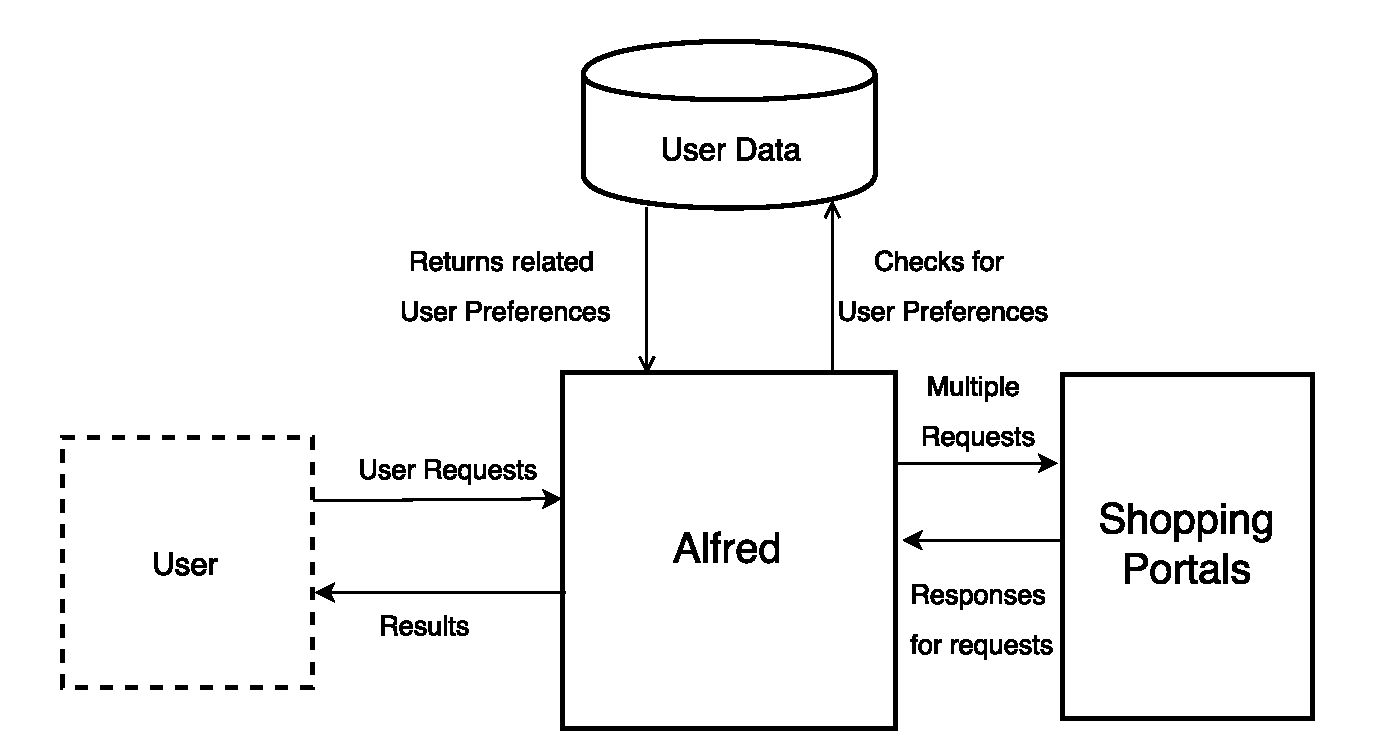
\includegraphics[width=0.5\textwidth]{Alfred}

\caption{Architecture of the Proposed System}
\end{figure}

The proposed system implements a number of sub-modules that collectively seek to overcome the chosen problem statement. These include seq2seq models to generate natural response utterances, NLP to understand and extract features from user input, query personalization to ensure that the products returned are relevant to the user and recommendation systems to deliver timely product recommendations.

The project will employ a sequential execution model, with the output of one stage passed as the input for the next stage. Figure 1 presents a high-level architecture of the proposed system. The user input is received and passed to the NLP module. The NLP stage will extract entities and parse the input to determine the user intent. This is then passed onto the query personalization stage. Using the available user profile, the possible search space for the result query is narrowed to maintain relevancy. The results of these queries are then presented to the user, who also has the option to generate recommendations on the basis of the returned result, on request.

The system employs an always-on learning mechanism, updating its knowledge base from time to time to stay up to date with the user's ever changing preferences. We propose that over time, such learning from a single user will help improve performance for all users.

\section{Proposed Methodology}

Figure 2 presents the flow of the proposed system. The proposed system will implement multiple modules that work together to deliver on the problem statement. \\

The NLP pipeline \cite{be7} is the first stage in the architecture and is the workhorse of the system. To understand user intent, the input is passed through a series of operations that are collectively referred to as the NLP pipeline.
\\


\begin{figure}

	\centering
	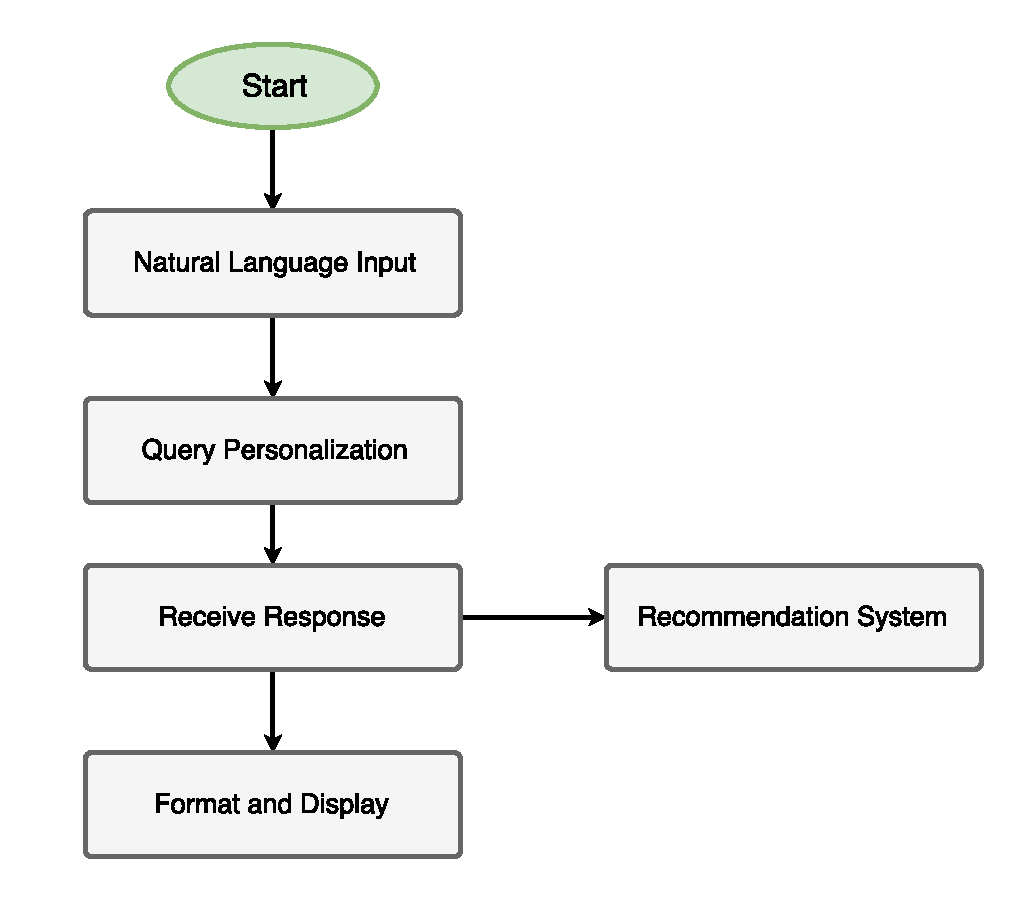
\includegraphics[width=0.50\textwidth]{flowchart.pdf}

\caption{Flow of the proposed system}
\end{figure}
\textbf{a. Tokenization} is often the first step in any NLP application and simply put, it is the process of chopping up the input into separate pieces called tokens. This helps us operate on the input one piece at a time, allowing our chatbot to understand context and construct word embeddings.

\textbf{b. Stop words removal} is a dimensionality reduction technique that helps in reducing the vector space of the input by eliminating words that are not essential. Stop words don\textquotesingle t add any domain information to the model and can be removed.

\textbf{c. Normalization} is the process of constructing canonical representations by applying linguistic models to tokens. This helps us group together tokens and entities that might seem different but refer to the same idea. Normalization includes the operations of Spell Checking and Lemmatization. 
\begin{itemize}
  \item Spell Checking: Each token is passed through a spell checker to allow the system to negate instances when the input is incorrectly typed or the speech processing wasn\textquotesingle ��t accurate.  
\end{itemize} 

\begin{itemize}
  \item Lemmatization: Lemmatization is the process of removing the inflectional and derivative forms of a word with the aim of returning the common base form of the word.
\end{itemize} 

\textbf{d. POS Tagging} is the process of reading a token and assigning a proper part of speech to it. This is an important task and helps us identify the user\textquotesingle s intentions by attaching POS tags to relevant keywords\cite{be13}.

\textbf{e. Named Entity Recognition} is the process of extracting named features from the input. This is helpful to further reduce the state space by focusing specifically on the named entities.

An initial query is first generated on the basis of results from the NLP subsystem. It is then passed through the query personalization module where the user\textquotesingle s profile comes in handy. By utilizing the available data, the system can ensure that the results generated by our system match the expectations of the user.

Query Personalization works by ensuring that the top preferences K of the user play a part in delivering the results. Once a minimum number L of these preferences are met, the query that satisfies the most number of preferences is chosen, giving a high degree of personalization\cite{be10}.

The proposed system uses a product assortment recommender that recommends and sorts a list of products on the basis of a user's preference. This is done by analyzing customer behaviour with the intention of arriving at two kinds of inferences: Associative Rules, so that product categories can be linked to each other and Collaborative Filtering, so that related brands can be linked within different product categories\cite{be12}. Collaborative Filtering works by building a matrix of preferences for users, and then matches that user with others in its neighbourhood given a similarity function.

\begin{equation}
{\textit{pred} = \frac{\overline{r} + \sum_{n \subset neighbours(u)}^ {}  sim_{(u,n)}^ { } * (r_{ni}^ {} -  \overline{r_{n}^ {}})} {sim_{(u,n)}^ {} * \sum_{n \subset neighbours(u)}^ {}}}
\end{equation}

For a given item \textit{i}, the algorithm will analyse the rating \textit{r} of other users \textit{u} in its similarity matrix. The similarity matrix is populated using the neighbourhood function \textbf{\textit{neighbours}} and uses the similarity function \textbf{sim} to generate the recommendation predictions \textbf{\textit{pred}}

\section{Results and Discussion}

This section deals with the performance of the proposed system and tries to evaluate its effectiveness against present approaches, on the basis of the following parameters:

\begin{itemize}
\item \textbf{Accuracy:} Measure of being correct with respect to shopping
\item \textbf{Effectiveness:} Completeness with which users achieve specified goals.
\item \textbf{Efficiency:} Resources expended in relation to the accuracy and completeness with which users achieve goals.
\item \textbf{Satisfaction:} Degree to which user needs are satisfied when a product or system is used in a specified context of use.
\end{itemize}

Accuracy is calculated on the basis of the following parameters
\begin{equation}
\textit{accuracy} = (w_j) * [p,e,r,c] 
\end{equation}
where each $w_j$ parameter is mapped to its respective attribute. \\


\begin{table*}[!ht]
\centering
\caption{Quality Model}
\label{my-label}
\begin{tabular}{@{}lllllllll@{}}
\toprule
User & Functional   & Stability   & Reliability &             & Performance & Efficiency & Usability   & Portability \\ \midrule
2    & 90.000000000 & 12.00310559 & 59.9        & 29.39440285 & 9.503186594 & 35.5       & 74.14920369 & 64.55648516 \\
5    & 92.00000000  & 77.62766177 & 61.9        & 32.99618284 & 16.20485038 & 40.5       & 73.33681143 & 62.41341209 \\
6    & 93.00000000  & 61.8951284  & 60.9        & 34.44990213 & 19.68624931 & 41.5       & 72.80185448 & 61.64720641 \\
7    & 93.00000000  & 61.8951284  & 61.3        & 36.07287146 & 23.4300375  & 44.3       & 72.16652471 & 62.14819377 \\
8    & 94.0000000   & 23.74054054 & 62          & 38.33138629 & 27.16342715 & 46.9       & 72.45639481 & 62.72306675 \\
9    & 91.00000000  & 25.84923973 & 62.5        & 40.11249564 & 30.52751868 & 49.9       & 73.19282134 & 63.61912216 \\
10   & 91.00000000  & 27.77047744 & 63.2        & 42.06555109 & 33.62163381 & 52.3       & 73.82114234 & 65.08838972 \\
19   & 94.00000000  & 77.62766177 & 61.7        & 50.09981147 & 46.7648277  & 60.4       & 77.62766177 & 67.14449816 \\
17   & 92.00000000  & 61.8951284  & 62.1        & 48.30067763 & 46.53291505 & 60         & 76.14301516 & 65.98256091 \\
12   & 92.00000000  & 29.84169408 & 63.3        & 45.24951206 & 39.26622984 & 56.4       & 75.84512345 & 65.83832154 \\
16   & 31.3796588   & 36.13334795 & 61.8        & 47.9098841  & 45.747782   & 59         & 75.92343971 & 65.79819852 \\
18   & 31.48642948  & 77.62766177 & 61.7        & 50.20987789 & 46.69046648 & 60.2       & 76.96309168 & 66.70603055 \\
20   & 31.6124031   & 61.8951284  & 62          & 50.77471585 & 46.7815648  & 60.5       & 78.11191872 & 67.01707156 \\
14   & 31.6353471   & 35.82625735 & 62.4        & 46.71313451 & 43.54206966 & 58.6       & 75.95060123 & 65.91837999 \\
13   & 32.63666364  & 34.81624758 & 63.1        & 45.96733794 & 41.94937335 & 58         & 75.84364914 & 65.84735212 \\
21   & 32.70344407  & 40.82404662 & 62.6        & 50.81809432 & 47.20085084 & 60.8       & 78.86685859 & 66.92190193 \\
23   & 33.93165961  & 35.20235628 & 61          & 51.34974154 & 47.21939541 & 59.7       & 78.43518191 & 65.62245655 \\
22   & 34.71183749  & 77.62766177 & 62.1        & 51.46880537 & 47.22432481 & 60.8       & 78.99124597 & 66.24147465 \\
25   & 36.03267447  & 34.43353129 & 59.4        & 52.2462176  & 47.98392441 & 58.1       & 75.81493264 & 65.64197772 \\
26   & 36.84480747  & 36.06321839 & 59.2        & 52.59940342 & 48.57318101 & 58.8       & 75.12525621 & 65.93694921 \\
27   & 38.96977475  & 35.9264854  & 58.6        & 53.78988011 & 48.6473926  & 58.7       & 75.03519921 & 66.43777883 \\
28   & 40.68568483  & 61.8951284  & 58.7        & 54.99946903 & 48.56105033 & 60         & 75.1637013  & 66.78635548 \\
29   & 41.91240333  & 77.62766177 & 59.1        & 56.35124789 & 49.2585152  & 60         & 75.48616027 & 67.2554484  \\
31   & 45.05776637  & 61.8951284  & 59.2        & 59.38985737 & 49.80361649 & 61.9       & 76.69214284 & 68.36599498 \\
32   & 45.86601517  & 61.8951284  & 59.4        & 60.71233149 & 50.27514494 & 63         & 77.37522931 & 68.57852029 \\
33   & 47.13465821  & 77.62766177 & 60.9        & 61.8951284  & 50.5523346  & 63.7       & 78.64424394 & 68.82995959 \\
39   & 47.570834    & 52.71173041 & 60.7        & 59.30576517 & 48.88802678 & 62.4       & 79.19632674 & 67.59402834 \\
38   & 47.60502633  & 43.10045895 & 61.4        & 59.41199314 & 49.00045935 & 62.5       & 78.72141311 & 67.87492278 \\
36   & 47.67275409  & 43.10036784 & 61.4        & 61.50098432 & 49.79185139 & 63.4       & 79.06712173 & 68.57122114 \\
35   & 47.88714025  & 92.46649345 & 61.3        & 61.91458697 & 49.95089449 & 64.2       & 78.65074774 & 68.45473436 \\
41   & 48.73004227  & 77.62766177 & 61.3        & 59.01025521 & 48.75798769 & 62.5       & 79.61862451 & 67.92810557 \\
1    & 70.00000000  & 77.62766177 & 59.7        & 29.08836297 & 9.064438975 & 35.3       & 74.53532758 & 65.57092343 \\
3    & 70.00000000  & 61.8951284  & 60.4        & 29.81022105 & 10.5589621  & 36.6       & 73.55451996 & 63.6642632  \\
4    & 69.00000000  & 61.8951284  & 60.2        & 31.14791477 & 12.80460152 & 38.4       & 73.50181443 & 62.94150212 \\
11   & 70.00000000  & 28.08038075 & 63.4        & 43.99925716 & 36.76572529 & 54.7       & 74.98103152 & 65.28413007 \\
15   & 67.00000000  & 92.00000000 & 62.1        & 47.66908276 & 45.12403027 & 59.1       & 75.86911601 & 65.74986233 \\
24   & 70.00000000  & 77.62766177 & 60.2        & 51.12484404 & 47.63933161 & 58.7       & 77.26731199 & 65.73095014 \\
30   & 70.00000000  & 38.63152919 & 59.2        & 58.22882288 & 49.81020815 & 61.2       & 75.83816206 & 67.82022113 \\
34   & 70.00000000  & 42.75854266 & 61.1        & 62.1694558  & 50.34559774 & 64.6       & 78.54494815 & 68.89448726 \\
37   & 73.00000000  & 79.62766177 & 61.6        & 60.17284465 & 49.21091439 & 63         & 78.68630551 & 68.29759443 \\
40   & 74.00000000  & 43.34892051 & 61          & 58.48958333 & 48.84047414 & 62.8       & 79.5329087  & 67.96979204 \\
42   & 72.00000000  & 61.8951284  & 61.2        & 58.7423969  & 48.18041792 & 62.2       & 79.43281184 & 68.42673015 \\ \bottomrule
\end{tabular}
\end{table*}




Here \textbf{\textit{p}} represents number of user preferences that are used, \textbf{\textit{e}} represents efficacy of generated recommendations, \textbf{\textit{r}} stands for the number of generated results and \textbf{\textit{c}} stands for the complexity of user query.

\begin{equation}
b_{4*4} = \begin{bmatrix}
    p_{11}       & p_{12} & p_{13} & p_{14} \\
    e_{21}       & e_{22} & e_{23} & e_{24} \\
    r_{31}       & r_{32} & r_{33} & r_{34} \\
    c_{41}       & c_{42} & c_{43} & c_{44}
\end{bmatrix}
\end{equation}

As per the Analytical Hierarchy Process Method\cite{be14}, the geometric mean can be used to represent individual normalized weights. The relative weights are then calculated by dividing each individual weight by the sum of weights, as given in equation 4 and 5

\begin{equation}
GM_j = [ \prod_{j=1}^{M} b_{ij}]^{1/M}
\end{equation}
where $b_{ij}$ represents the comparison matrix as defined in equation 3.
\begin{center}
and 
\end{center}
\begin{equation}
w_j = GM_j / \sum_{j=1}^{M} GM_j
\end{equation}

After performing the above analysis, the weights have been calculated to be as follows:
p = 0.4, e = 0.3, r = 0.2, c = 0.1 rounded off to nearest significant digit.

\begin{figure}[h!]

	\centering
	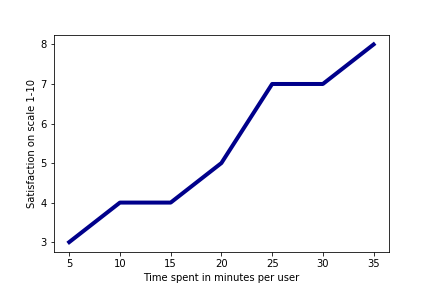
\includegraphics[width=0.5\textwidth]{Time-Spent}

\caption{Time-Satisfaction Plot}
\end{figure}

Satisfaction = \textit{k}, where \textit{k} represents user satisfaction at time \textit{i}  \\

Figure 3 represents the satisfaction level of users, mapped over a continuous time interval. A sample set of users of the assistant indicated higher levels of satisfaction with increasing time, indicating that the assistant had learnt to tailor itself to the particular user. 

\begin{table}[]
\centering
\caption{Time Spent}
\label{my-label}
\begin{tabular}{||l|l|l|l|l|l|l|l||}
\hline
0  & 0  & 0  & 1  & 4  & 7   & 8  & 8   \\ \hline
1  & 5  & 5  & 3  & 0  & 6   & 6  & 7   \\
2  & 3  & 3  & 5  & 6  & 5   & 10 & 10  \\
3  & 7  & 7  & 2  & 9  & 9   & 9  & 10  \\
4  & 3  & 3  & 3  & 6  & 7   & 8  & 8   \\
5  & 4  & 4  & 3  & 5  & 5   & 7  & 7   \\
6  & 1  & 1  & 8  & 7  & 6   & 8  & 7   \\
7  & 1  & 1  & 0  & 9  & 6   & 8  & 8   \\
8  & 3  & 3  & 6  & 8  & 5   & 5  & 7   \\
9  & 1  & 1  & 10 & 6  & 8   & 6  & 8   \\
10 & 6  & 6  & 1  & 6  & 5   & 5  & 8   \\
11 & 2  & 2  & 1  & 2  & 6   & 10 & 10  \\
12 & 2  & 2  & 7  & 6  & 9   & 5  & 9   \\
13 & 2  & 2  & 2  & 9  & 8   & 5  & 10  \\
14 & 6  & 6  & 4  & 4  & 9   & 7  & 10  \\
15 & 7  & 7  & 6  & 4  & 10  & 8  & 7   \\
16 & 4  & 4  & 6  & 1  & 8   & 7  & 9   \\
17 & 2  & 2  & 6  & 8  & 9   & 5  & 9   \\
18 & 0  & 0  & 0  & 3  & 5   & 6  & 7   \\
19 & 1  & 1  & 1  & 1  & 6   & 9  & 7   \\
20 & 0  & 0  & 9  & 3  & 6   & 9  & 9   \\
21 & 0  & 0  & 0  & 4  & 5   & 10 & 8   \\
22 & 9  & 9  & 8  & 2  & 10  & 7  & 10  \\
23 & 4  & 4  & 0  & 3  & 10  & 5  & 10  \\
24 & 2  & 2  & 5  & 0  & 10  & 9  & 7   \\
25 & 5  & 5  & 1  & 0  & 8   & 5  & 7   \\
26 & 10 & 10 & 6  & 7  & 6   & 8  & 10  \\
27 & 5  & 5  & 0  & 7  & 6   & 6  & 10  \\
28 & 4  & 4  & 4  & 8  & 5   & 6  & 7   \\
29 & 7  & 7  & 8  & 9  & 3.9 & 2  & 1.3 \\ \hline
\end{tabular}
\end{table}

\begin{figure}

	\centering
	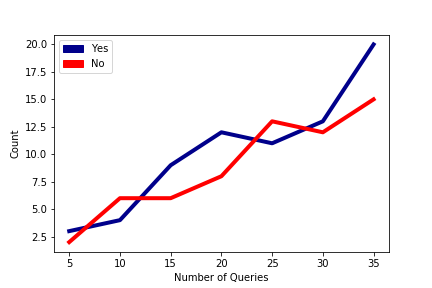
\includegraphics[width=0.50\textwidth]{Effectiveness.png}

\caption{Effectiveness Plot}
\end{figure}

Figure 4 represents the effectiveness of the assistant over time, as indicated by users. For a particular session, the user rates the effectiveness of each operation on the basis of fulfilment of the task.

$Count_{no}^ { }$ and $Count_{yes}^ { }$ represents the number of positive and negative operations as indicated by the user.
\section{Conclusion}

In this paper, we proposed an automated shopping assistant, which is efficient and utilizes Natural Language Processing and modern interfaces  to make online shopping convenient. The assistant also understands the user's specific preferences and helps them buy products that they are likely to enjoy. Most existing systems use partially automated systems and are do not deliver intelligent recommendations. Future work will involve focusing on general purpose queries and consider non-behavioural data points to arrive at intelligent recommendation. 

\begin{thebibliography}{99}

\bibitem{be1}
Victor Zue, James Glass, Conversational Interfaces: Advantages and Challenges, Proceedings of the IEEE, Vol. 88, No. 8, 1166-1180, August 2000

\bibitem{be2}
Victor Zue, Stephanie Seneff, James Glass, Joseph Polifroni, Christine Pao, Timothy Hazen, Lee Hetherington, JUPITER - A Telephone based Conversational Interface, IEEE Transactions on Speech and Audio Processing, Vol. 8, No. 1, January 2000

\bibitem{be3}
Ilya Sutskever, Oriol Vinyals, Quoc V. Lee, Sequence to Sequence Learning with Neural Networks, Neural Information Processing Systems, Montreal 2014

\bibitem{be4}
A Conversational Interface for Online Shopping \\
\url{http://www.aclweb.org/anthology/H01-1012 }

\bibitem{be5}
S. Quarteroni, S. Manandhar, Designing an Interactive Open-Domain Question Answering System, Natural Language Engineeirng, Volume 15, Issue 1, 73-95

\bibitem{be6}
Ryuichiro Higashinaka, Kenji Imamura, Toyomi Meguro, Chiaki Miyazaki, Nozomi Kobayashi, Hiroaki Sugiyama, Toru Hirano, Toshiro Makino, Yoshihiro Matsuo, Proceedings of COLING 2014, the 25th International Conference on Computational Linguistics: Technical Papers, 928-939

\bibitem{be7}
Giuseppe Attardi, DeepNL: A Deep Learning NLP Pipeline, Proceedings of the $1^{st}$ workshop on Vector Space Modeling for Natural Language Processing, June 2015

\bibitem{be8} 
The Learning Chatbot \\
\url{http://courses.ischool.berkeley.edu/i256/f06/projects/bonniejc.pdf}

\bibitem{be9}
Cold Fusion: Training Seq2Seq models together with language models, arXiv preprint \\
\url{http://arxiv.org/pdf/1708.06426.pdf}

\bibitem{be10}
Georgia Koutrika, Yannis Ioannidis, Query Personalization based on User Preferences, Dagstuhl Seminar Proceedings\\
\url{http://drops.dagstuhl.de/opus/volltexte/2006/403/pdf/04271.KoutrikaGeorgia.Paper.403.pdf}

\bibitem{be11}
George Prassas, Katherine Pramatris, Olga Papaeammanouil, Georgios Doukidis, A Recommender System for Online Shopping based on Past Customer Behaviour, 14th Bled Electronics Commerce Conference, June 2001

\bibitem{be12}
Jonathan Herlocker, Joseph Konstan, Loren Terveen, John Riedl, Evaluating Collaborative Filtering Recommendation Systems, ACM Transactions on Information Systems 22, 5-33, January 2004

\bibitem{be13}
Kevin Gimpel, Nathan Schneider, Brendan O'Connor, Dipanjan Das, Daniel Mills, Jacob Eisenstein, Michael Heilman, Dani Yogatama, Jeffrey Flanigan, and Noah A. Smith, Part-of-Speech Tagging for Twitter: Annotation, Features and experiments, Proceedings of the 49th Annual Meeting of the Association for Computational Linguistics: Human Language Technologies: Short Papers - Volume 2, 42-47.

\bibitem{be14}
Michalewicz Z., Schmidt M., Michalewicz M., Chiriac C, Adaptive Business Intelligence, 2006, Springer-Verlag Berlin Heidelberg
\end{thebibliography}
 
\end{document}
